% !TeX TS-program = xelatex
% !BIB TS-program = bibtex

% Full instructions available at:
% https://github.com/elauksap/focus-beamertheme

\documentclass[aspectratio=169]{beamer}
\setbeamerfont{footnote}{size=\tiny}
\setbeamerfont{caption}{size=\tiny}
\setbeamerfont{block title}{size=\large}
\setbeamerfont{block body}{size=\small}
\usetheme[numbering=minimal,nofirafonts,totalframenumbering=no]{focus}
% \definecolor{main}{RGB}{82, 82, 82}
\definecolor{main}{RGB}{37, 37, 37}
\definecolor{background}{RGB}{247, 247, 247}
\usepackage{biblatex}
\addbibresource{report.bib}
\usepackage{booktabs}
\usepackage{caption}
\captionsetup{labelformat=empty}

\title{Data vs. Model Centric ML Fairness Testing}
\subtitle{An Empirical Study}
\author{Arumoy Shome\texorpdfstring{\\}{,} Lu{\'\i}s
  Cruz\texorpdfstring{\\}Arie van Deursen}
\institute{Delft University of Technology}
\date{\today}

% Footline info is printed only if [numbering=fullbar].
%\footlineinfo{Custom footline text}

\begin{document}
\begin{frame}
  \maketitle
\end{frame}

% Use starred version (e.g. \section*{Section name})
% to disable (sub)section page.
\section{Introduction}

\begin{frame}{Testing non-deterministic ML systems is challenging\ldots}
  \begin{enumerate}
    \item ML is being adopted in high-risk domains (healthcare,
      finance and criminal justice)
    \item ability to impact human-lives
    \item concerns being raised toward trust, robustness, privacy,
      security and fairness
    \item preference given to testing for robustness and correctness
      (security, privacy, efficiency, \textbf{\emph{interpretability}}
      and \textbf{\emph{fairness}}) have been ignored
  \end{enumerate}
\end{frame}
\begin{frame}[focus]
  \emph{Conduct a preliminary exploratory study to evaluate the
  effectiveness of fairness testing both before and after model
  training.}
\end{frame}

\section{Preliminaries}

\begin{frame}{Algorithmic bias}
  \begin{columns}[t, onlytextwidth]
    \column{0.5\linewidth}
    \begin{center}
      \textbf{But what is fair?}
    \end{center}
    \begin{itemize}
      \item Fairness is a multi-facet, socio-technical problem and
        currently an open challenge in ML
      \item Perils of manual label validation\ldots
      \item Quantify bias using fairness metrics
    \end{itemize}

    \column{0.5\linewidth}
    \begin{center}
      \textbf{Fairness metrics}
    \end{center}
    \begin{itemize}
        \item limited to supervised binary classification
        \item one label is favourable than the other (qualify for loan
          or not)
        \item protected attribute in dataset (such as \emph{race, sex, age,
          colour, religion or disability status}
        \item one group is privileged while the other is unprivileged
          (more examples of male vs. female)
    \end{itemize}
  \end{columns}
\end{frame}

\begin{frame}{Individual vs. group fairness}
  \begin{columns}[t, onlytextwidth]
    \column{0.5\linewidth}
    \begin{center}
      \textbf{Individual fairness}
    \end{center}

    Predictions for two similar individuals differing only in the
    protected attribute should be similar.
    \column{0.5\linewidth}
    \begin{center}
      \textbf{Group fairness}
    \end{center}

    Predictions for two groups in the protected attribute should be
    similar.
  \end{columns}
\end{frame}

\begin{frame}{Bias mitigation techniques}
  \begin{columns}[t, onlytextwidth]
    \column{0.33\linewidth}
    \begin{center}
      \textbf{Pre-processing techniques}
    \end{center}
    Mitigate bias in the training data (over/under sampling,
    reweighting, etc.)
    \column{0.33\linewidth}
    \begin{center}
      \textbf{In-processing techniques}
    \end{center}
    ML algorithms that consider fairness while training from biased
    data.
    \column{0.33\linewidth}
    \begin{center}
      \textbf{Post-processing techniques}
    \end{center}
    Mitigate bias in the predictions of the model.
  \end{columns}
\end{frame}

\section{Experimental Design}
\setbeamertemplate{caption}[numbered]
\begin{frame}{Datasets used in this study}
  \begin{table}
    \centering
    \caption{Datasets used in the study}
    \begin{tabular}{llr}
      \toprule
      \textbf{Name} & \textbf{Prot.} & \textbf{Total Examples}\\
      \midrule
      German Credit \footfullcite{hofmann1994german} & age, sex & 1000\\
      Compas Score \footfullcite{angwin2016machine} & race, sex & 6167\\
      Medical Survey 2021 \footfullcite{mepsdata} & race & 15675\\
      Bank Marketing \footfullcite{moro2014data} & age & 30488\\
      Adult Income \footfullcite{kohavi1996scaling} & race, sex & 45222\\
      \bottomrule
    \end{tabular}
    \label{tab:datasets}
  \end{table}
\end{frame}

\begin{frame}{ML models used in this study}
  \begin{itemize}
    \item Logistic Regression (LR)
    \item Decision Trees (DT)
    \item Random Forest (RF)
    \item Ada Boost (ADA)
  \end{itemize}
\end{frame}

\begin{frame}[t]{Group Fairness Metrics used in this study}
  \begin{center}
    \textbf{Before training}
  \end{center}
  \begin{equation}
    DI_{data} = \frac{P(Y=1|D=0)}{P(Y=1|D=1)}
    \label{eq:di-data}
  \end{equation}

  \begin{equation}
    SPD_{data} = P(Y=1|D=0)-P(Y=1|D=1)
    \label{eq:spd-data}
  \end{equation}

  \vfill

  \begin{center}
    \textbf{After training}
  \end{center}
  \begin{equation}
    DI_{model} = \frac{P(\hat{Y}=1|D=0)}{P(\hat{Y}=1|D=1)}
    \label{eq:di-model}
  \end{equation}

  \begin{equation}
    SPD_{model} = P(\hat{Y}=1|D=0)-P(\hat{Y}=1|D=1)
    \label{eq:spd-model}
  \end{equation}
\end{frame}

\begin{frame}{Fairness evaluation}
  \begin{figure}[c]
    \centering
    \includegraphics[width=0.95\linewidth]{method.pdf}
    \caption{Methodology for data collection and analysis}
    \label{fig:method}
  \end{figure}
\end{frame}

\begin{frame}{Parameters of this study}
  \begin{table}
    \centering
    \begin{tabular}{lr}
      \toprule
      \textbf{Parameter} & \textbf{Count}\\
      \midrule
      Fairness metrics & 2\\
      ML models & 4\\
      Datasets & 8\\
      Total cases & $8*4=32$\\
      Iterations & 50\\
      Total fairness evaluation cycles & $32*50=1600$\\
      \bottomrule
    \end{tabular}
    \label{tab:parameters}
    \caption{Parameters of the study}
  \end{table}
\end{frame}

\section{Results}
\begin{frame}{Overview of Results}
  \begin{columns}[t]
    \column{0.5\textwidth}
    \begin{center}
      \textbf{Full training set experiments}
    \end{center}
    \begin{enumerate}
    \item What is the relationship between DFM and MFM?
    \item What is the relationship between DFM and MFM as the
      underlying data distribution changes?
    \item How does the training sample size affect the relationship
      between DFM and MFM?
    \end{enumerate}
    \column{0.5\textwidth}
    \begin{center}
      \textbf{Training and feature sample size experiments}
    \end{center}
    \begin{enumerate}
    \item What is the relationship between DFM and MFM across training
      sample sizes?
    \item What is the relationship between DFM and MFM across
      feature sample sizes?
    \end{enumerate}
  \end{columns}
\end{frame}

\subsection{Full training set experiments}
\begin{frame}{What is the relationship between DFM and MFM?}
  \begin{figure}
    \centering
    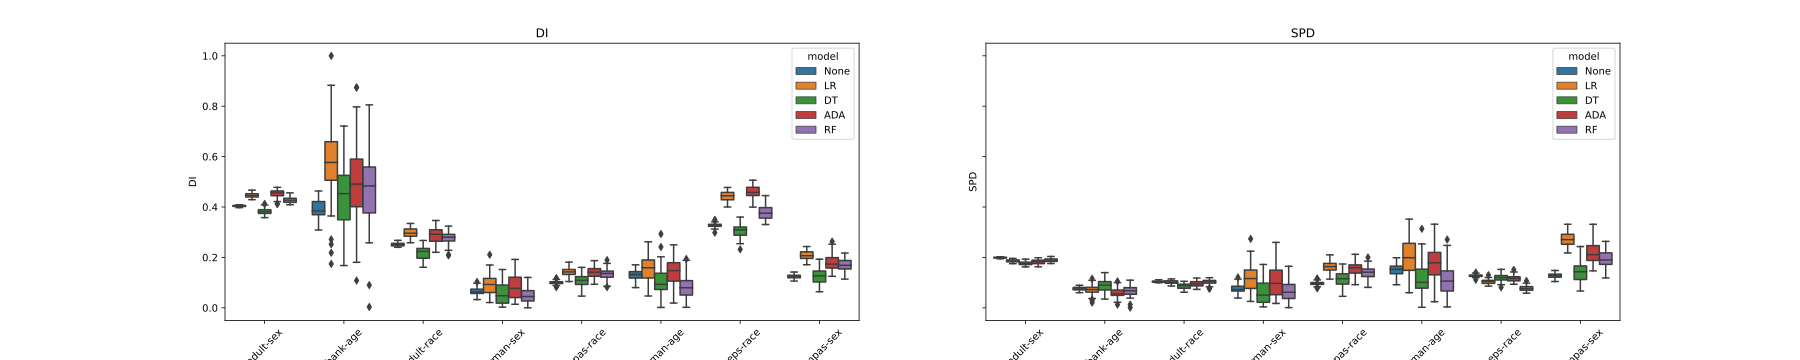
\includegraphics[width=0.7\textwidth,height=0.45\textheight]{boxplot--dataset--di-spd--exp-full.pdf}
    \caption{Distribution of DFM and MFM across datasets}
    \label{fig:boxplot--dataset--di-spd--exp-full}
  \end{figure}

  \begin{exampleblock}{DFM and MFM convey similar information in all
    cases}
      Variability of $DFM < MFM$
  \end{exampleblock}
\end{frame}

\begin{frame}{What is the relationship between DFM and MFM?}
  \begin{figure}
    \centering
    \includegraphics[width=0.95\linewidth]{heatmap--corr--full-data.pdf}
    \caption{Correlation between DFM and MFM}
    \label{fig:heatmap--corr--full-data}
  \end{figure}

  \begin{alertblock}{No correlation between DFM and MFM in most cases}
    No significant change in the underlying distribution of the
    training set.
  \end{alertblock}
\end{frame}

\begin{frame}{What is the relationship between DFM and MFM as the
  underlying data distribution changes?}
  \begin{columns}[t, onlytextwidth]
    \column{0.55\textwidth}
    \begin{figure}
      \centering
      \includegraphics[width=0.95\textwidth]{training-set-frac-threshold.pdf}
      \caption{\emph{\textbf{(left)}} Accuracy and f1 across various
        training sample size in german-age \emph{\textbf{(right)}} Number
        of cases with significant change in accuracy and f1}
      \label{fig:training-set-frac-threshold}
    \end{figure}

    \column{0.4\textwidth}
    \begin{block}{Introduce (more) change in distribution of training data}
      \begin{itemize}
        \item \emph{student-t test} to check significant change
          between different training sample sizes
        \item 60\% training sample size produces significant
          distribution change with acceptable performance
      \end{itemize}
    \end{block}
  \end{columns}
\end{frame}

\begin{frame}{What is the relationship between DFM and MFM as the
  underlying data distribution changes?}
  \begin{figure}
    \centering
    \includegraphics[width=0.95\linewidth]{heatmap--corr--training-sets-frac.pdf}
    \caption{Correlation between DFM and MFM across all models and
      datasets using 60\% training data}
    \label{fig:heatmap--corr--training-sets-frac}
  \end{figure}

  \begin{exampleblock}{Positive correlation between DFM and MFM in
    majority of cases}
    DFM and MFM convey the same information as distribution of
    training set changes.
  \end{exampleblock}
\end{frame}

\begin{frame}{How does the training sample size affect the
    relationship between DFM and MFM?}
    \begin{columns}[c, onlytextwidth]
      \column{0.55\textwidth}
      \begin{figure}
        \centering
        \includegraphics[width=0.95\textwidth]{lineplot--frac--corr.pdf}
        \caption{Distribution of correlation between DFM and MFM across
          various training sample sizes}
        \label{fig:lineplot--frac--corr}
      \end{figure}

      \column{0.4\textwidth}
      \begin{exampleblock}{Quantity of training data affects
        relationship between DFM and MFM}
        Correlation between DFM and MFM \alert{decreases} as we
        \textcolor{example}{increase} the training size.
      \end{exampleblock}
    \end{columns}
\end{frame}

\subsection{Training and feature sets experiments}

\begin{frame}{What is the relationship between DFM and MFM across
  various training samples?}
  \begin{figure}
    \centering
    \includegraphics[width=0.95\linewidth]{heatmap--corr--frac.pdf}
    \caption{Correlation between DFM and MFM acoss various training
      sample sizes}
    \label{fig:heatmap--corr--frac}
  \end{figure}
\end{frame}

\begin{frame}{What is the relationship between DFM and MFM across
  various feature samples? [1/2]}
  \begin{figure}
    \centering
    \includegraphics[width=0.95\linewidth]{heatmap--corr--num-features.pdf}
    \caption{Correlation between DFM and MFM across various feature
      sample sizes}
    \label{fig:heatmap--corr--num-features}
  \end{figure}
\end{frame}

\begin{frame}{What is the relationship between DFM and MFM across
  various feature samples? [2/2]}
  \begin{figure}
    \centering
    \includegraphics[height=0.7\textheight, keepaspectratio]{lineplot--num-features--corr.pdf}
    \caption{Distribution of correlation between DFM and MFM across
      various features sample sizes}
    \label{fig:lineplot--num-features--corr}
  \end{figure}
\end{frame}

\section{Discussion} % (fold)

\begin{frame}{Locating root cause of bias}
  \begin{exampleblock}{A holistic view of the entire system is
    necessary to locate the root cause of bias}
    \begin{itemize}
      \item \emph{DFM indicates bias}: early indication of flaws in
        initial software design or biased data collection process
      \item \emph{DFM does not indicate bias but MFM does}: cause of
        bias in the learning algorithm itself
    \end{itemize}
  \end{exampleblock}
\end{frame}

\begin{frame}{Fairness, efficiency and performance trade-off}
  \begin{figure}
    \centering
    \includegraphics[height=0.7\textheight, keepaspectratio]{lineplot--frac--corr.pdf}
    \caption{Distribution of correlation between DFM and MFM across
      various training sample sizes}
  \end{figure}
\end{frame}

\begin{frame}{Fairness, efficiency and performance trade-off}
  \begin{exampleblock}{Positive correlation}
    \begin{itemize}
      \item may indicate lack of sufficient training data
      \item either get more training data or use bias mitigation
        techniques
    \end{itemize}
  \end{exampleblock}

  \begin{alertblock}{Negative correlation ($MFM<DFM$)}
    \begin{itemize}
      \item bias in data not reflected in model (but there yet be
        bias!)
      \item efficiency vs. performance trade-off
      \item engineering high quality, high quality training data can
        \textcolor{example}{reduce} training cycles, time and
        ultimately project costs.
    \end{itemize}
  \end{alertblock}

  \begin{block}{No correlation}
    \begin{itemize}
      \item fairness vs. efficiency vs. performance trade-off
    \end{itemize}
  \end{block}
\end{frame}

\begin{frame}{Data drift}
  \begin{figure}
    \centering
    \includegraphics[width=0.95\linewidth]{heatmap--corr--training-sets-frac.pdf}
    \caption{Correlation between DFM and MFM across all models and
      datasets using 60\% training data}
  \end{figure}

  \begin{exampleblock}{DFM can be an early indication of fairness
    issues that may manifest in the ML models when the distribution of
    the training data changes}
    DFM can be an early warning system to identify fairness related
    data drifts in automated ML pipelines.
  \end{exampleblock}
\end{frame}

\begin{frame}[t]{Test Reduction}
  \begin{columns}[t, onlytextwidth]
    \column{0.5\textwidth}
    \begin{figure}
      \centering
      \includegraphics[height=0.2\textheight, keepaspectratio]{heatmap--corr--frac.pdf}
      \caption{Correlation between DFM and MFM acoss various training
        sample sizes}
    \end{figure}

    \column{0.5\textwidth}
    \begin{figure}
      \centering
      \includegraphics[height=0.2\textheight, keepaspectratio]{heatmap--corr--num-features.pdf}
      \caption{Correlation between DFM and MFM across various feature
        sample sizes}
    \end{figure}
  \end{columns}

  \vfill

  \begin{exampleblock}{Testing can be reduced to just training data
    when experimenting with training sample size}
    The same however \alert{cannot} be done when experimenting with
    feature sample size.
  \end{exampleblock}
\end{frame}

\begin{frame}{Explaining fairness in decision trees}
  \begin{figure}
    \centering
    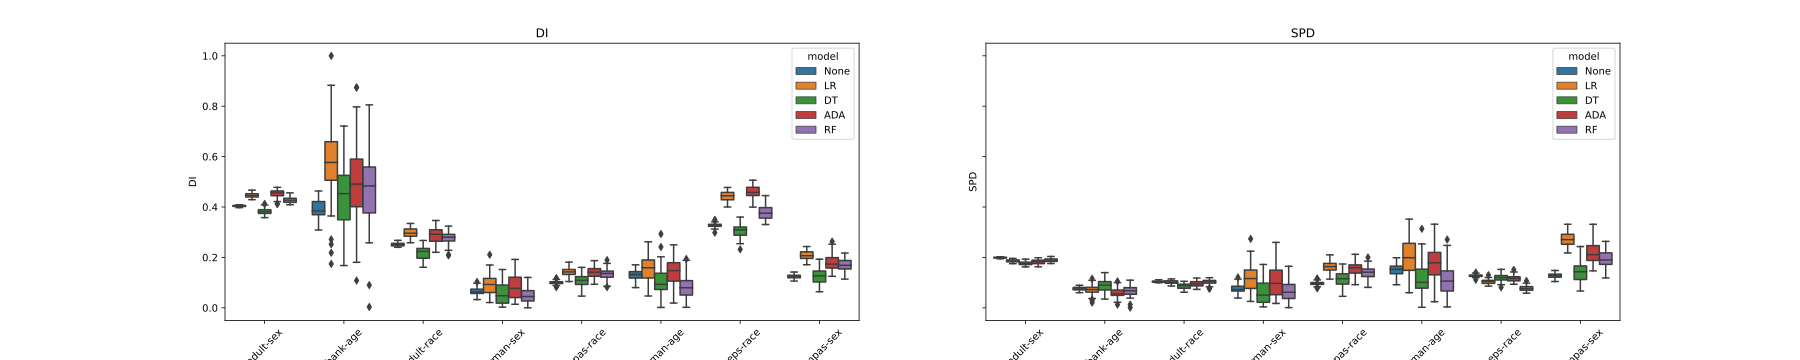
\includegraphics[height=0.7\textheight,keepaspectratio]{boxplot--dataset--di-spd--exp-full.pdf}
    \caption{Distribution of DFM and MFM across datasets}
  \end{figure}
\end{frame}

\begin{frame}{Explaining fairness in decision trees}
  \begin{figure}
    \centering
    \includegraphics[height=0.7\textheight, keepaspectratio]{lineplot--frac--corr.pdf}
    \caption{Distribution of correlation between DFM and MFM across
      various training sample sizes}
  \end{figure}
\end{frame}

\begin{frame}{Explaining fairness in decision trees}
  \begin{exampleblock}{DTs consistently make fairer predictions with
    minimal effort}
    \begin{itemize}
      \item Can we examine why DTs are able to produce fairner
        predictions using Explainable AI techniques?
    \end{itemize}
  \end{exampleblock}
\end{frame}

\section{Concluding Remarks} % (fold)

\begin{frame}{Threats to validity}
  \begin{itemize}
    \item 
  \end{itemize}
\end{frame}

\begin{frame}{Thank you}
  \begin{itemize}
    \item Fully reproducible and openly accessible replication
      package (coming soon!)
    \item Feedback? Questions? Concerns?: \emph{a.shome@tudelft.nl}
    \item Github: \emph{arumoy-shome}
    \item Project website:
      \emph{https://arumoy.me/shome2022qualitative} (coming soon!)
  \end{itemize}
\end{frame}
% section Concluding Remarks (end)

% section Discussion (end)
% \appendix
% \begin{frame}{References}
%   \nocite{*}
%   \bibliography{report}
%   \bibliographystyle{named}
% \end{frame}
\end{document}
